\section{INSAT-3D Sounder Polychromatic Correction Temperature Fit Residuals}
%============================================================================
\label{app.sndr_tfit_data_plots}

\subsection{Channel 1}
\begin{figure}[H]
  \label{fig:sndr_ch1_tfit}
  \centering
  \begin{tabular}{c}
    \includegraphics[scale=0.55]{graphics/sndr/tfit/sndr_insat3d-1.tfit.eps} \\
    \includegraphics[scale=0.55]{graphics/sndr/tfit/sndr_insat3d-1.tfit.difference.eps}
  \end{tabular}
  \caption{INSAT-3D Sounder channel 1 polychromatic correction temperature fit residuals. \emph{(Top)} Comparison of residuals for original and new SRFs. \emph{(Bottom)} Residual differences for the original and new SRFs.}
\end{figure}

\subsection{Channel 2}
\begin{figure}[H]
  \label{fig:sndr_ch2_tfit}
  \centering
  \begin{tabular}{c}
    \includegraphics[scale=0.55]{graphics/sndr/tfit/sndr_insat3d-2.tfit.eps} \\
    \includegraphics[scale=0.55]{graphics/sndr/tfit/sndr_insat3d-2.tfit.difference.eps}
  \end{tabular}
  \caption{INSAT-3D Sounder channel 2 polychromatic correction temperature fit residuals. \emph{(Top)} Comparison of residuals for original and new SRFs. \emph{(Bottom)} Residual differences for the original and new SRFs.}
\end{figure}

\subsection{Channel 3}
\begin{figure}[H]
  \label{fig:sndr_ch3_tfit}
  \centering
  \begin{tabular}{c}
    \includegraphics[scale=0.55]{graphics/sndr/tfit/sndr_insat3d-3.tfit.eps} \\
    \includegraphics[scale=0.55]{graphics/sndr/tfit/sndr_insat3d-3.tfit.difference.eps}
  \end{tabular}
  \caption{INSAT-3D Sounder channel 3 polychromatic correction temperature fit residuals. \emph{(Top)} Comparison of residuals for original and new SRFs. \emph{(Bottom)} Residual differences for the original and new SRFs.}
\end{figure}

\subsection{Channel 4}
\begin{figure}[H]
  \label{fig:sndr_ch4_tfit}
  \centering
  \begin{tabular}{c}
    \includegraphics[scale=0.55]{graphics/sndr/tfit/sndr_insat3d-4.tfit.eps} \\
    \includegraphics[scale=0.55]{graphics/sndr/tfit/sndr_insat3d-4.tfit.difference.eps}
  \end{tabular}
  \caption{INSAT-3D Sounder channel 4 polychromatic correction temperature fit residuals. \emph{(Top)} Comparison of residuals for original and new SRFs. \emph{(Bottom)} Residual differences for the original and new SRFs.}
\end{figure}

\subsection{Channel 5}
\begin{figure}[H]
  \label{fig:sndr_ch5_tfit}
  \centering
  \begin{tabular}{c}
    \includegraphics[scale=0.55]{graphics/sndr/tfit/sndr_insat3d-5.tfit.eps} \\
    \includegraphics[scale=0.55]{graphics/sndr/tfit/sndr_insat3d-5.tfit.difference.eps}
  \end{tabular}
  \caption{INSAT-3D Sounder channel 5 polychromatic correction temperature fit residuals. \emph{(Top)} Comparison of residuals for original and new SRFs. \emph{(Bottom)} Residual differences for the original and new SRFs.}
\end{figure}

\subsection{Channel 6}
\begin{figure}[H]
  \label{fig:sndr_ch6_tfit}
  \centering
  \begin{tabular}{c}
    \includegraphics[scale=0.55]{graphics/sndr/tfit/sndr_insat3d-6.tfit.eps} \\
    \includegraphics[scale=0.55]{graphics/sndr/tfit/sndr_insat3d-6.tfit.difference.eps}
  \end{tabular}
  \caption{INSAT-3D Sounder channel 6 polychromatic correction temperature fit residuals. \emph{(Top)} Comparison of residuals for original and new SRFs. \emph{(Bottom)} Residual differences for the original and new SRFs.}
\end{figure}

\subsection{Channel 7}
\begin{figure}[H]
  \label{fig:sndr_ch7_tfit}
  \centering
  \begin{tabular}{c}
    \includegraphics[scale=0.55]{graphics/sndr/tfit/sndr_insat3d-7.tfit.eps} \\
    \includegraphics[scale=0.55]{graphics/sndr/tfit/sndr_insat3d-7.tfit.difference.eps}
  \end{tabular}
  \caption{INSAT-3D Sounder channel 7 polychromatic correction temperature fit residuals. \emph{(Top)} Comparison of residuals for original and new SRFs. \emph{(Bottom)} Residual differences for the original and new SRFs.}
\end{figure}

\subsection{Channel 8}
\begin{figure}[H]
  \label{fig:sndr_ch8_tfit}
  \centering
  \begin{tabular}{c}
    \includegraphics[scale=0.55]{graphics/sndr/tfit/sndr_insat3d-8.tfit.eps} \\
    \includegraphics[scale=0.55]{graphics/sndr/tfit/sndr_insat3d-8.tfit.difference.eps}
  \end{tabular}
  \caption{INSAT-3D Sounder channel 8 polychromatic correction temperature fit residuals. \emph{(Top)} Comparison of residuals for original and new SRFs. \emph{(Bottom)} Residual differences for the original and new SRFs.}
\end{figure}

\subsection{Channel 9}
\begin{figure}[H]
  \label{fig:sndr_ch9_tfit}
  \centering
  \begin{tabular}{c}
    \includegraphics[scale=0.55]{graphics/sndr/tfit/sndr_insat3d-9.tfit.eps} \\
    \includegraphics[scale=0.55]{graphics/sndr/tfit/sndr_insat3d-9.tfit.difference.eps}
  \end{tabular}
  \caption{INSAT-3D Sounder channel 9 polychromatic correction temperature fit residuals. \emph{(Top)} Comparison of residuals for original and new SRFs. \emph{(Bottom)} Residual differences for the original and new SRFs.}
\end{figure}

\subsection{Channel 10}
\begin{figure}[H]
  \label{fig:sndr_ch10_tfit}
  \centering
  \begin{tabular}{c}
    \includegraphics[scale=0.55]{graphics/sndr/tfit/sndr_insat3d-10.tfit.eps} \\
    \includegraphics[scale=0.55]{graphics/sndr/tfit/sndr_insat3d-10.tfit.difference.eps}
  \end{tabular}
  \caption{INSAT-3D Sounder channel 10 polychromatic correction temperature fit residuals. \emph{(Top)} Comparison of residuals for original and new SRFs. \emph{(Bottom)} Residual differences for the original and new SRFs.}
\end{figure}

\subsection{Channel 11}
\begin{figure}[H]
  \label{fig:sndr_ch11_tfit}
  \centering
  \begin{tabular}{c}
    \includegraphics[scale=0.55]{graphics/sndr/tfit/sndr_insat3d-11.tfit.eps} \\
    \includegraphics[scale=0.55]{graphics/sndr/tfit/sndr_insat3d-11.tfit.difference.eps}
  \end{tabular}
  \caption{INSAT-3D Sounder channel 11 polychromatic correction temperature fit residuals. \emph{(Top)} Comparison of residuals for original and new SRFs. \emph{(Bottom)} Residual differences for the original and new SRFs.}
\end{figure}

\subsection{Channel 12}
\begin{figure}[H]
  \label{fig:sndr_ch12_tfit}
  \centering
  \begin{tabular}{c}
    \includegraphics[scale=0.55]{graphics/sndr/tfit/sndr_insat3d-12.tfit.eps} \\
    \includegraphics[scale=0.55]{graphics/sndr/tfit/sndr_insat3d-12.tfit.difference.eps}
  \end{tabular}
  \caption{INSAT-3D Sounder channel 12 polychromatic correction temperature fit residuals. \emph{(Top)} Comparison of residuals for original and new SRFs. \emph{(Bottom)} Residual differences for the original and new SRFs.}
\end{figure}

\subsection{Channel 13}
\begin{figure}[H]
  \label{fig:sndr_ch13_tfit}
  \centering
  \begin{tabular}{c}
    \includegraphics[scale=0.55]{graphics/sndr/tfit/sndr_insat3d-13.tfit.eps} \\
    \includegraphics[scale=0.55]{graphics/sndr/tfit/sndr_insat3d-13.tfit.difference.eps}
  \end{tabular}
  \caption{INSAT-3D Sounder channel 13 polychromatic correction temperature fit residuals. \emph{(Top)} Comparison of residuals for original and new SRFs. \emph{(Bottom)} Residual differences for the original and new SRFs.}
\end{figure}

\subsection{Channel 14}
\begin{figure}[H]
  \label{fig:sndr_ch14_tfit}
  \centering
  \begin{tabular}{c}
    \includegraphics[scale=0.55]{graphics/sndr/tfit/sndr_insat3d-14.tfit.eps} \\
    \includegraphics[scale=0.55]{graphics/sndr/tfit/sndr_insat3d-14.tfit.difference.eps}
  \end{tabular}
  \caption{INSAT-3D Sounder channel 14 polychromatic correction temperature fit residuals. \emph{(Top)} Comparison of residuals for original and new SRFs. \emph{(Bottom)} Residual differences for the original and new SRFs.}
\end{figure}

\subsection{Channel 15}
\begin{figure}[H]
  \label{fig:sndr_ch15_tfit}
  \centering
  \begin{tabular}{c}
    \includegraphics[scale=0.55]{graphics/sndr/tfit/sndr_insat3d-15.tfit.eps} \\
    \includegraphics[scale=0.55]{graphics/sndr/tfit/sndr_insat3d-15.tfit.difference.eps}
  \end{tabular}
  \caption{INSAT-3D Sounder channel 15 polychromatic correction temperature fit residuals. \emph{(Top)} Comparison of residuals for original and new SRFs. \emph{(Bottom)} Residual differences for the original and new SRFs.}
\end{figure}

\subsection{Channel 16}
\begin{figure}[H]
  \label{fig:sndr_ch16_tfit}
  \centering
  \begin{tabular}{c}
    \includegraphics[scale=0.55]{graphics/sndr/tfit/sndr_insat3d-16.tfit.eps} \\
    \includegraphics[scale=0.55]{graphics/sndr/tfit/sndr_insat3d-16.tfit.difference.eps}
  \end{tabular}
  \caption{INSAT-3D Sounder channel 16 polychromatic correction temperature fit residuals. \emph{(Top)} Comparison of residuals for original and new SRFs. \emph{(Bottom)} Residual differences for the original and new SRFs.}
\end{figure}

\subsection{Channel 17}
\begin{figure}[H]
  \label{fig:sndr_ch17_tfit}
  \centering
  \begin{tabular}{c}
    \includegraphics[scale=0.55]{graphics/sndr/tfit/sndr_insat3d-17.tfit.eps} \\
    \includegraphics[scale=0.55]{graphics/sndr/tfit/sndr_insat3d-17.tfit.difference.eps}
  \end{tabular}
  \caption{INSAT-3D Sounder channel 17 polychromatic correction temperature fit residuals. \emph{(Top)} Comparison of residuals for original and new SRFs. \emph{(Bottom)} Residual differences for the original and new SRFs.}
\end{figure}

\subsection{Channel 18}
\begin{figure}[H]
  \label{fig:sndr_ch18_tfit}
  \centering
  \begin{tabular}{c}
    \includegraphics[scale=0.55]{graphics/sndr/tfit/sndr_insat3d-18.tfit.eps} \\
    \includegraphics[scale=0.55]{graphics/sndr/tfit/sndr_insat3d-18.tfit.difference.eps}
  \end{tabular}
  \caption{INSAT-3D Sounder channel 18 polychromatic correction temperature fit residuals. \emph{(Top)} Comparison of residuals for original and new SRFs. \emph{(Bottom)} Residual differences for the original and new SRFs.}
\end{figure}
